\section{Messergebnisse und Auswertung}
\subsection{Peltierelement}

\begin{figure}[H]
\begin{center}
  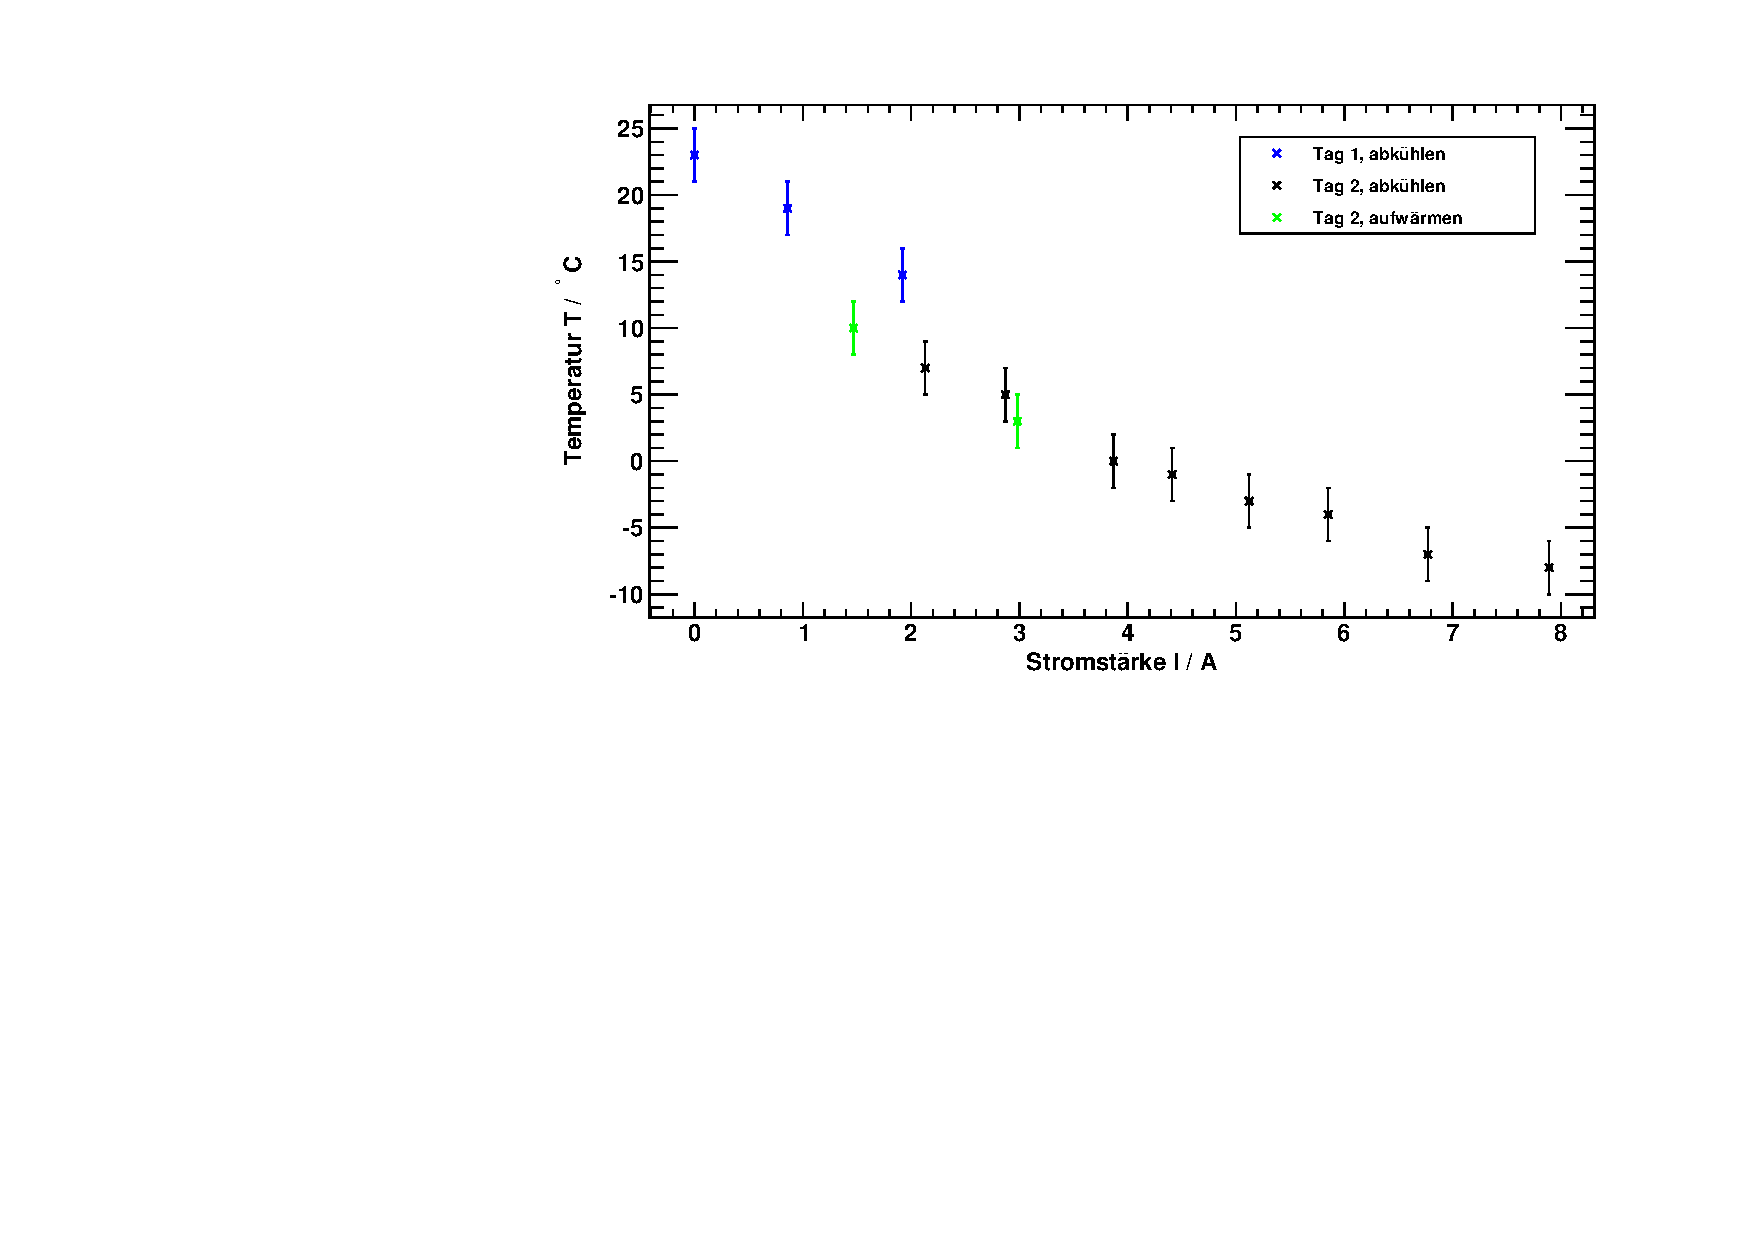
\includegraphics[width=\textwidth]{../img/graph_T-I.pdf}
  \caption{Temperatur am Thermoelement
  in Abhängigkeit des Stroms durch das Peltierelement.}
  \label{img:TI}
\end{center}
\end{figure}

\autoref{img:TI} zeigt den Zusammenhang zwischen Strom durch das Peltierelement
und der Temperatur, die sich nach 30 Minuten Stromfluss am Thermoelement eingestellt hat.
Es ist ein exponentieller Verlauf mit Sättigung bei hohem Strom zu erkennen.
Dies kann mit dem Wärmefluss aus der Umgebung begründet werden.
Auf einen Fit wurde hier verzichtet, da die genaue Information über den Zusammenhang
für die Auswertung nicht relevant ist.
Man erkennt allerdings, dass die Messwerte für Abkühlung (schwarz) und Erwärmung (grün) konsistent sind.
Die Einschwingzeit von 30 Minuten ist also lang genug gewählt.
Zwischen 1. und 2. Messtag besteht ein großer Offset.
Dies könnte an der Temperatur des Kühlwassers liegen,
das am ersten Tag von einem anderen Verbraucher im Haus erwärmt wurde.\\
\autoref{img:UI} zeigt die Strom-Spannungs-Kennlinie des Peltierelements.
Der Zusammenhang ist linear, der Widerstand beträgt über den gesamten Arbeitsbereich ca. 3\,\textOmega.
Die Kühlleistung des Elements ist also sowohl zum Quadrat des Stroms als auch zum Quadrat der Spannung proportional.



\begin{figure}[H]
\begin{center}
  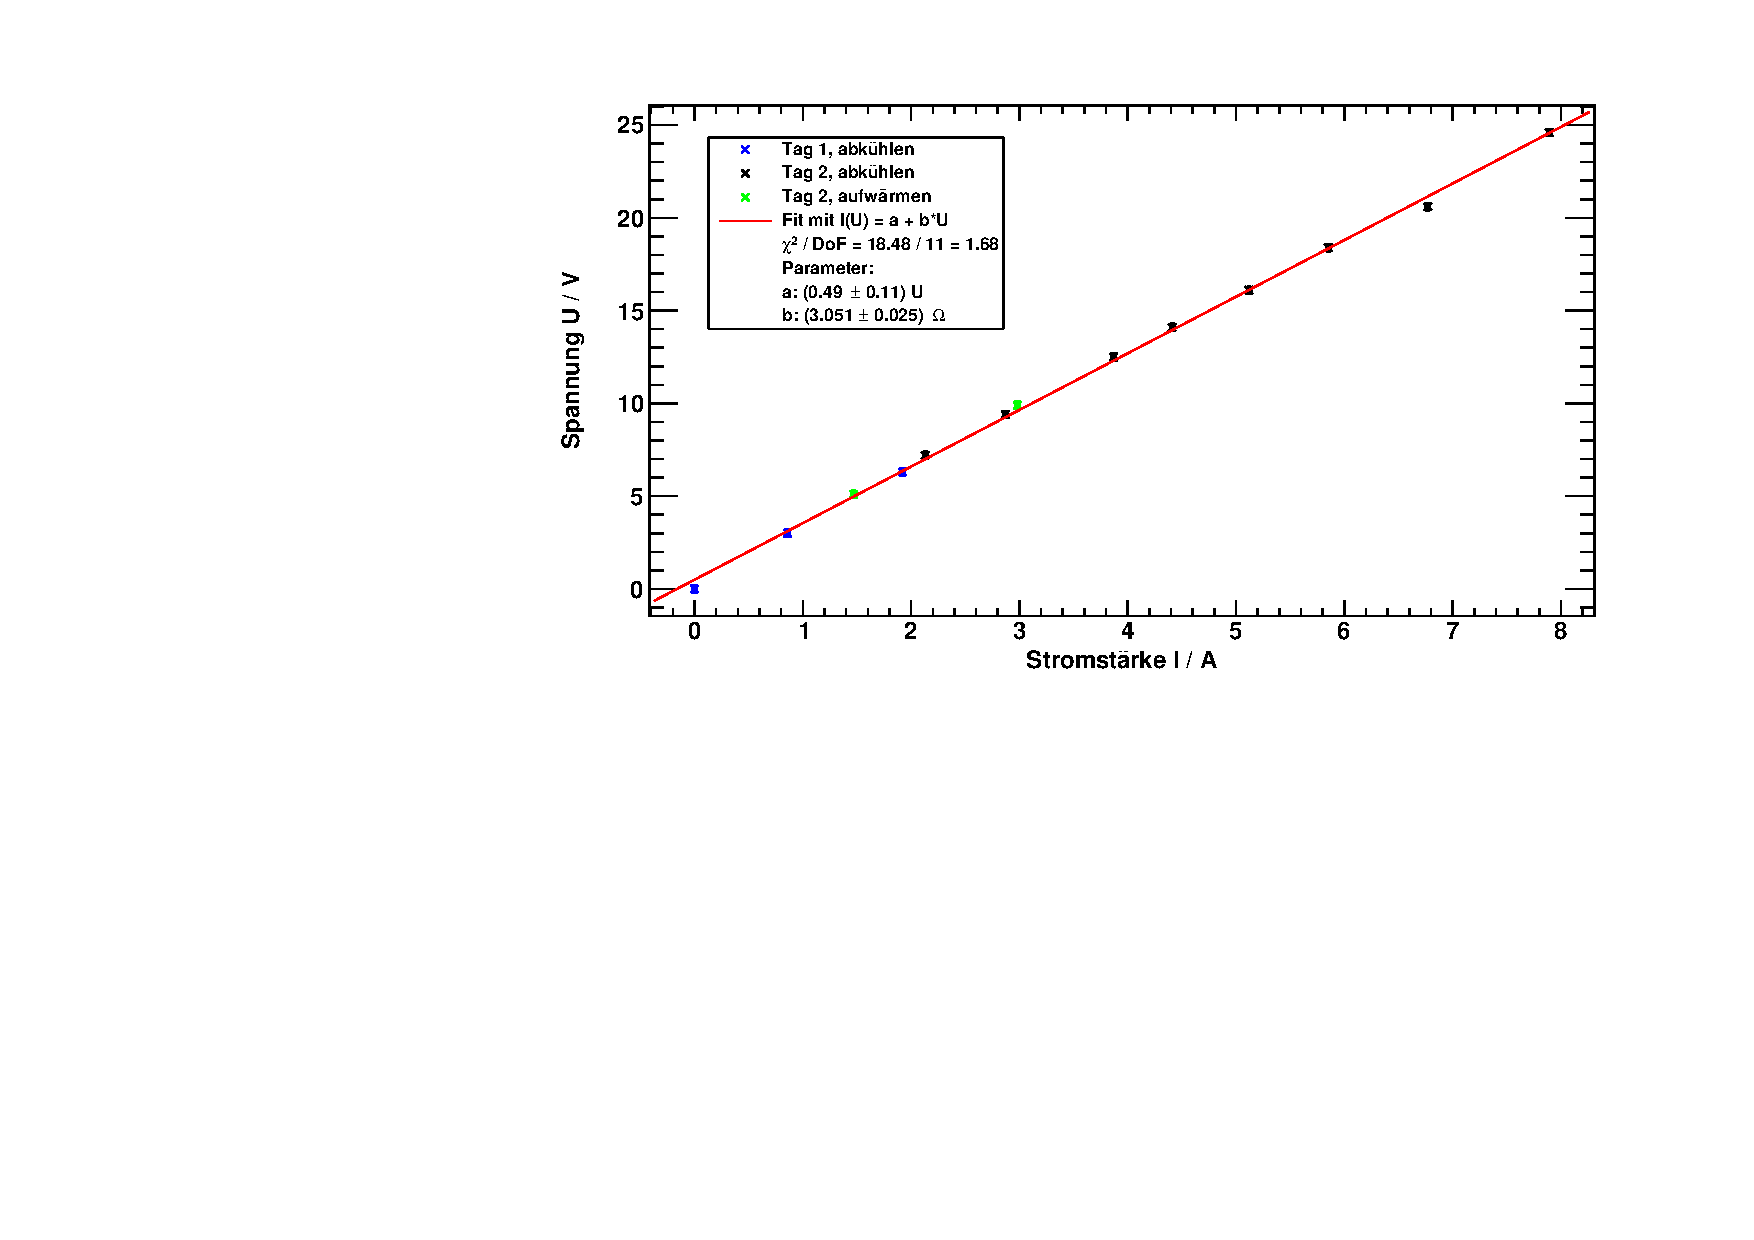
\includegraphics[width=\textwidth]{../img/graph_U-I.pdf}
  \caption{Strom-Spannungs-Kennlinie des Peltierelements.}
  \label{img:UI}
\end{center}
\end{figure}




\subsection{Bestimmung der Lebensdauer aus dem Lorentz-Peak}
Ausgewähltes Beispiel
\subsection{Fehler auf die Lebensdauer}
\subsection{Extrapolation auf 0 Pa}